% Options for packages loaded elsewhere
\PassOptionsToPackage{unicode}{hyperref}
\PassOptionsToPackage{hyphens}{url}
\PassOptionsToPackage{dvipsnames,svgnames,x11names}{xcolor}
%
\documentclass[
  a4paper,
]{report}

\usepackage{amsmath,amssymb}
\usepackage{lmodern}
\usepackage{iftex}
\ifPDFTeX
  \usepackage[T1]{fontenc}
  \usepackage[utf8]{inputenc}
  \usepackage{textcomp} % provide euro and other symbols
\else % if luatex or xetex
  \usepackage{unicode-math}
  \defaultfontfeatures{Scale=MatchLowercase}
  \defaultfontfeatures[\rmfamily]{Ligatures=TeX,Scale=1}
  \setmainfont[]{NanumMyeongjo}
  \setsansfont[]{NanumGothic}
  \setmonofont[]{D2Coding}
\fi
% Use upquote if available, for straight quotes in verbatim environments
\IfFileExists{upquote.sty}{\usepackage{upquote}}{}
\IfFileExists{microtype.sty}{% use microtype if available
  \usepackage[]{microtype}
  \UseMicrotypeSet[protrusion]{basicmath} % disable protrusion for tt fonts
}{}
\makeatletter
\@ifundefined{KOMAClassName}{% if non-KOMA class
  \IfFileExists{parskip.sty}{%
    \usepackage{parskip}
  }{% else
    \setlength{\parindent}{0pt}
    \setlength{\parskip}{6pt plus 2pt minus 1pt}}
}{% if KOMA class
  \KOMAoptions{parskip=half}}
\makeatother
\usepackage{xcolor}
\setlength{\emergencystretch}{3em} % prevent overfull lines
\setcounter{secnumdepth}{5}
% Make \paragraph and \subparagraph free-standing
\ifx\paragraph\undefined\else
  \let\oldparagraph\paragraph
  \renewcommand{\paragraph}[1]{\oldparagraph{#1}\mbox{}}
\fi
\ifx\subparagraph\undefined\else
  \let\oldsubparagraph\subparagraph
  \renewcommand{\subparagraph}[1]{\oldsubparagraph{#1}\mbox{}}
\fi

\usepackage{color}
\usepackage{fancyvrb}
\newcommand{\VerbBar}{|}
\newcommand{\VERB}{\Verb[commandchars=\\\{\}]}
\DefineVerbatimEnvironment{Highlighting}{Verbatim}{commandchars=\\\{\}}
% Add ',fontsize=\small' for more characters per line
\usepackage{framed}
\definecolor{shadecolor}{RGB}{241,243,245}
\newenvironment{Shaded}{\begin{snugshade}}{\end{snugshade}}
\newcommand{\AlertTok}[1]{\textcolor[rgb]{0.68,0.00,0.00}{#1}}
\newcommand{\AnnotationTok}[1]{\textcolor[rgb]{0.37,0.37,0.37}{#1}}
\newcommand{\AttributeTok}[1]{\textcolor[rgb]{0.40,0.45,0.13}{#1}}
\newcommand{\BaseNTok}[1]{\textcolor[rgb]{0.68,0.00,0.00}{#1}}
\newcommand{\BuiltInTok}[1]{\textcolor[rgb]{0.00,0.23,0.31}{#1}}
\newcommand{\CharTok}[1]{\textcolor[rgb]{0.13,0.47,0.30}{#1}}
\newcommand{\CommentTok}[1]{\textcolor[rgb]{0.37,0.37,0.37}{#1}}
\newcommand{\CommentVarTok}[1]{\textcolor[rgb]{0.37,0.37,0.37}{\textit{#1}}}
\newcommand{\ConstantTok}[1]{\textcolor[rgb]{0.56,0.35,0.01}{#1}}
\newcommand{\ControlFlowTok}[1]{\textcolor[rgb]{0.00,0.23,0.31}{#1}}
\newcommand{\DataTypeTok}[1]{\textcolor[rgb]{0.68,0.00,0.00}{#1}}
\newcommand{\DecValTok}[1]{\textcolor[rgb]{0.68,0.00,0.00}{#1}}
\newcommand{\DocumentationTok}[1]{\textcolor[rgb]{0.37,0.37,0.37}{\textit{#1}}}
\newcommand{\ErrorTok}[1]{\textcolor[rgb]{0.68,0.00,0.00}{#1}}
\newcommand{\ExtensionTok}[1]{\textcolor[rgb]{0.00,0.23,0.31}{#1}}
\newcommand{\FloatTok}[1]{\textcolor[rgb]{0.68,0.00,0.00}{#1}}
\newcommand{\FunctionTok}[1]{\textcolor[rgb]{0.28,0.35,0.67}{#1}}
\newcommand{\ImportTok}[1]{\textcolor[rgb]{0.00,0.46,0.62}{#1}}
\newcommand{\InformationTok}[1]{\textcolor[rgb]{0.37,0.37,0.37}{#1}}
\newcommand{\KeywordTok}[1]{\textcolor[rgb]{0.00,0.23,0.31}{#1}}
\newcommand{\NormalTok}[1]{\textcolor[rgb]{0.00,0.23,0.31}{#1}}
\newcommand{\OperatorTok}[1]{\textcolor[rgb]{0.37,0.37,0.37}{#1}}
\newcommand{\OtherTok}[1]{\textcolor[rgb]{0.00,0.23,0.31}{#1}}
\newcommand{\PreprocessorTok}[1]{\textcolor[rgb]{0.68,0.00,0.00}{#1}}
\newcommand{\RegionMarkerTok}[1]{\textcolor[rgb]{0.00,0.23,0.31}{#1}}
\newcommand{\SpecialCharTok}[1]{\textcolor[rgb]{0.37,0.37,0.37}{#1}}
\newcommand{\SpecialStringTok}[1]{\textcolor[rgb]{0.13,0.47,0.30}{#1}}
\newcommand{\StringTok}[1]{\textcolor[rgb]{0.13,0.47,0.30}{#1}}
\newcommand{\VariableTok}[1]{\textcolor[rgb]{0.07,0.07,0.07}{#1}}
\newcommand{\VerbatimStringTok}[1]{\textcolor[rgb]{0.13,0.47,0.30}{#1}}
\newcommand{\WarningTok}[1]{\textcolor[rgb]{0.37,0.37,0.37}{\textit{#1}}}

\providecommand{\tightlist}{%
  \setlength{\itemsep}{0pt}\setlength{\parskip}{0pt}}\usepackage{longtable,booktabs,array}
\usepackage{calc} % for calculating minipage widths
% Correct order of tables after \paragraph or \subparagraph
\usepackage{etoolbox}
\makeatletter
\patchcmd\longtable{\par}{\if@noskipsec\mbox{}\fi\par}{}{}
\makeatother
% Allow footnotes in longtable head/foot
\IfFileExists{footnotehyper.sty}{\usepackage{footnotehyper}}{\usepackage{footnote}}
\makesavenoteenv{longtable}
\usepackage{graphicx}
\makeatletter
\def\maxwidth{\ifdim\Gin@nat@width>\linewidth\linewidth\else\Gin@nat@width\fi}
\def\maxheight{\ifdim\Gin@nat@height>\textheight\textheight\else\Gin@nat@height\fi}
\makeatother
% Scale images if necessary, so that they will not overflow the page
% margins by default, and it is still possible to overwrite the defaults
% using explicit options in \includegraphics[width, height, ...]{}
\setkeys{Gin}{width=\maxwidth,height=\maxheight,keepaspectratio}
% Set default figure placement to htbp
\makeatletter
\def\fps@figure{htbp}
\makeatother
\newlength{\cslhangindent}
\setlength{\cslhangindent}{1.5em}
\newlength{\csllabelwidth}
\setlength{\csllabelwidth}{3em}
\newlength{\cslentryspacingunit} % times entry-spacing
\setlength{\cslentryspacingunit}{\parskip}
\newenvironment{CSLReferences}[2] % #1 hanging-ident, #2 entry spacing
 {% don't indent paragraphs
  \setlength{\parindent}{0pt}
  % turn on hanging indent if param 1 is 1
  \ifodd #1
  \let\oldpar\par
  \def\par{\hangindent=\cslhangindent\oldpar}
  \fi
  % set entry spacing
  \setlength{\parskip}{#2\cslentryspacingunit}
 }%
 {}
\usepackage{calc}
\newcommand{\CSLBlock}[1]{#1\hfill\break}
\newcommand{\CSLLeftMargin}[1]{\parbox[t]{\csllabelwidth}{#1}}
\newcommand{\CSLRightInline}[1]{\parbox[t]{\linewidth - \csllabelwidth}{#1}\break}
\newcommand{\CSLIndent}[1]{\hspace{\cslhangindent}#1}

\usepackage{pdfpages}
\makeatletter
\@ifpackageloaded{tcolorbox}{}{\usepackage[many]{tcolorbox}}
\@ifpackageloaded{fontawesome5}{}{\usepackage{fontawesome5}}
\definecolor{quarto-callout-color}{HTML}{909090}
\definecolor{quarto-callout-note-color}{HTML}{0758E5}
\definecolor{quarto-callout-important-color}{HTML}{CC1914}
\definecolor{quarto-callout-warning-color}{HTML}{EB9113}
\definecolor{quarto-callout-tip-color}{HTML}{00A047}
\definecolor{quarto-callout-caution-color}{HTML}{FC5300}
\definecolor{quarto-callout-color-frame}{HTML}{acacac}
\definecolor{quarto-callout-note-color-frame}{HTML}{4582ec}
\definecolor{quarto-callout-important-color-frame}{HTML}{d9534f}
\definecolor{quarto-callout-warning-color-frame}{HTML}{f0ad4e}
\definecolor{quarto-callout-tip-color-frame}{HTML}{02b875}
\definecolor{quarto-callout-caution-color-frame}{HTML}{fd7e14}
\makeatother
\makeatletter
\makeatother
\makeatletter
\makeatother
\makeatletter
\@ifpackageloaded{caption}{}{\usepackage{caption}}
\AtBeginDocument{%
\ifdefined\contentsname
  \renewcommand*\contentsname{Table of contents}
\else
  \newcommand\contentsname{Table of contents}
\fi
\ifdefined\listfigurename
  \renewcommand*\listfigurename{List of Figures}
\else
  \newcommand\listfigurename{List of Figures}
\fi
\ifdefined\listtablename
  \renewcommand*\listtablename{List of Tables}
\else
  \newcommand\listtablename{List of Tables}
\fi
\ifdefined\figurename
  \renewcommand*\figurename{Figure}
\else
  \newcommand\figurename{Figure}
\fi
\ifdefined\tablename
  \renewcommand*\tablename{Table}
\else
  \newcommand\tablename{Table}
\fi
}
\@ifpackageloaded{float}{}{\usepackage{float}}
\floatstyle{ruled}
\@ifundefined{c@chapter}{\newfloat{codelisting}{h}{lop}}{\newfloat{codelisting}{h}{lop}[chapter]}
\floatname{codelisting}{Listing}
\newcommand*\listoflistings{\listof{codelisting}{List of Listings}}
\makeatother
\makeatletter
\@ifpackageloaded{caption}{}{\usepackage{caption}}
\@ifpackageloaded{subcaption}{}{\usepackage{subcaption}}
\makeatother
\makeatletter
\@ifpackageloaded{tcolorbox}{}{\usepackage[many]{tcolorbox}}
\makeatother
\makeatletter
\@ifundefined{shadecolor}{\definecolor{shadecolor}{rgb}{.97, .97, .97}}
\makeatother
\makeatletter
\@ifpackageloaded{sidenotes}{}{\usepackage{sidenotes}}
\@ifpackageloaded{marginnote}{}{\usepackage{marginnote}}
\makeatother
\makeatletter
\makeatother
\ifLuaTeX
  \usepackage{selnolig}  % disable illegal ligatures
\fi
\IfFileExists{bookmark.sty}{\usepackage{bookmark}}{\usepackage{hyperref}}
\IfFileExists{xurl.sty}{\usepackage{xurl}}{} % add URL line breaks if available
\urlstyle{same} % disable monospaced font for URLs
\hypersetup{
  pdftitle={한글 LaTeX},
  pdfauthor={이광춘},
  colorlinks=true,
  linkcolor={blue},
  filecolor={Maroon},
  citecolor={Blue},
  urlcolor={Blue},
  pdfcreator={LaTeX via pandoc}}

\title{한글 LaTeX}
\author{이광춘}
\date{}

\begin{document}
\maketitle
\ifdefined\Shaded\renewenvironment{Shaded}{\begin{tcolorbox}[enhanced, borderline west={3pt}{0pt}{shadecolor}, sharp corners, breakable, frame hidden, interior hidden, boxrule=0pt]}{\end{tcolorbox}}\fi

\renewcommand*\contentsname{Table of contents}
{
\hypersetup{linkcolor=}
\setcounter{tocdepth}{1}
\tableofcontents
}
\begin{tcolorbox}[enhanced jigsaw, opacityback=0, coltitle=black, left=2mm, colframe=quarto-callout-caution-color-frame, breakable, rightrule=.15mm, colbacktitle=quarto-callout-caution-color!10!white, colback=white, bottomtitle=1mm, toptitle=1mm, leftrule=.75mm, toprule=.15mm, titlerule=0mm, opacitybacktitle=0.6, title=\textcolor{quarto-callout-caution-color}{\faFire}\hspace{0.5em}{Danger}, arc=.35mm, bottomrule=.15mm]
\href{https://aispiration.com/ds-authoring/ct-writing.html}{이광춘,
``글을 쓰는 것은 소프트웨어 개발이다!'', 강서양천신문 특집기고('15년
9월)} 와 \href{http://aispiration.com/latex/}{LaTeX, PDF, 문서, 그리고
사고}에서 관련 내용을 발췌한 것임을 밝혀둡니다. 그리고,
\href{https://quarto.org/docs/output-formats/pdf-basics.html}{Quarto
PDF} 문서를 많이 참고 했습니다.
\end{tcolorbox}

\hypertarget{uxcd9cuxd310-uxb514uxc9c0uxd138-uxc804uxd658}{%
\chapter{출판 디지털
전환}\label{uxcd9cuxd310-uxb514uxc9c0uxd138-uxc804uxd658}}

200자 원고지 4장은 통상 A4 용지 한장에 해당한다. 만약 A4 용지 10장
보고서나 논문을 작성한다고 하면, 종이 200자 원고지 40장에 연필이나
볼펜을 가지고 작성하게 된다. 최종본을 얻기까지 빨간색으로 선생님이나
주변의 첨삭지도를 받아 최종본을 만들기까지 여러번의 반복과정을 거치게
된다.

최종 원고가 200자 원고지 40장에 담겨 탈고를 마치게 되면, 독자에게 다가갈
준비를 한다. 그림을 넣거나 아름다운 글씨체를 적용해 보고 종이 재질을
바꿔보기도 하고 영혼이 담긴 원고를 독자가 보기 좋고, 이해하기 쉽고,
때로는 감동과 재미를 줄 수 있도록 출판 단계에서 많은 사람들의 노력이
들어간다.

탈고를 마친 원고에 글씨체를 비롯한 디자인 작업이 완료되면 출판장비를
갖춘 출판소에서 인쇄장비를 거쳐 종이책 혹은 보고서가 완성되고, 이렇게
대량으로 출력되면 각 서점으로 배송되어 독자가 서점에서 구독을 하게 된다.

저자의 생각을 글로 표현하면 현재도 대부분 편집 및 디자인, 출판, 배송,
서점 등 각 단계에 사람이 관여하고 필요에 따라서는 컴퓨터가 작업을
지원하는데 사용되어 최종 독자에게 전달된다.

책과 보고서 제작하는 과정은 워드 프로세스를 기본으로 두고, 숫자 계산이
필요하면 엑셀, 이미지가 필요하면 그래픽 전문 소프트웨어, 정보 검색도
웹브라우져를 사용한다. 글자, 단어, 문장, 문단, 장/절/항으로 생각의
단위를 서문, 본문, 결어 및 참고문헌, 주석, 그림, 그래프, 도표 등도 함께
체계적으로 작성해 나간다.

다양한 소프트웨어를 통해서 원고를 탈고하게 되면 서식, 문장 문단 모양,
색인, 참조문헌 등 보기 좋고 가독성 높은 형태로 외양을 입히는 과정을
거치게 되는데 이 과정도 소프트웨어가 핵심적인 역할을 하게 된다. 책과
보고서에 대한 디자인 작업이 완료되면 다양한 형태로 배포하기 위한
프로그래밍 과정을 거쳐 PDF, 전자책(ePUB), 웹(HTML), 출판책 형태로
독자에게 전달된다.

글을 써서 이를 독자에게 전달되는 과정은 과거에 전문작가, 디자인 전문가,
출판전문가, 서점운영자 등 수많은 전문가가 연관되어 있고 타자기, 디자인
기계, 인쇄기 등 수많은 기계가 필요했으며 이를 사업적으로 기술적으로
연결할 수 있는 다양한 통신 방법이 필요했다. 비전문가가 밖에서 보면
복잡하고 어려워 보이지만, 컴퓨팅 사고의 시각으로 보면 단순할 수 있다.

\hypertarget{uxc544uxb0a0uxb85cuxadf8-uxcd9cuxd310}{%
\subsubsection{아날로그
출판}\label{uxc544uxb0a0uxb85cuxadf8-uxcd9cuxd310}}

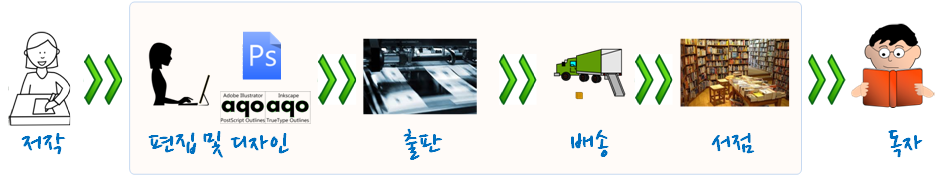
\includegraphics{fig/pdf-analog.png}

\hypertarget{uxb514uxc9c0uxd138-uxcd9cuxd310}{%
\subsubsection{디지털 출판}\label{uxb514uxc9c0uxd138-uxcd9cuxd310}}

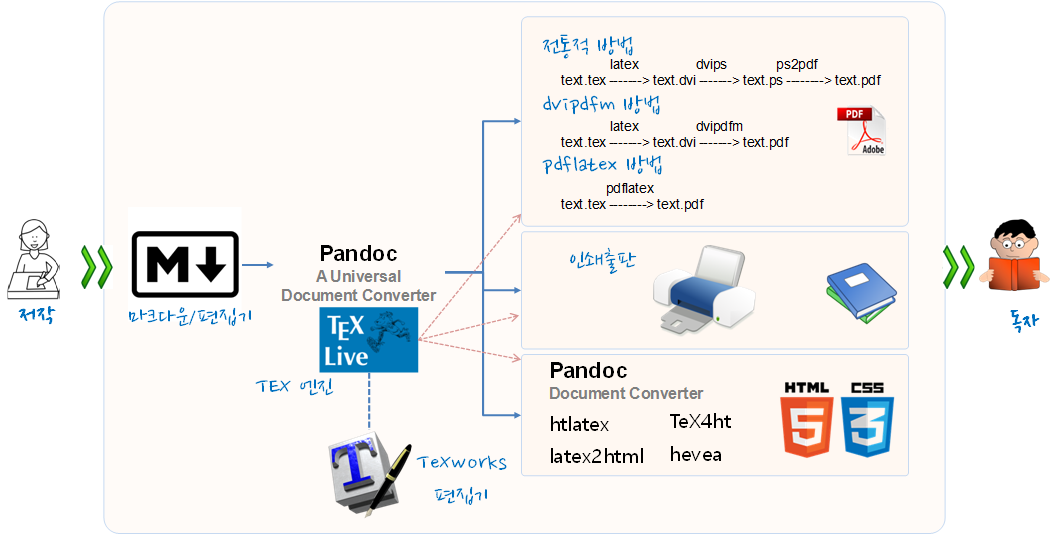
\includegraphics{fig/pdf-digital.png}

\hypertarget{quarto-pdf}{%
\chapter{Quarto PDF}\label{quarto-pdf}}

PDF는 기술적, 학술적, 사업적으로 혁신적인 문서 양식이다. PDF가 개발된
것은 오랜 역사를 자랑하지만 아래한글, 워드퍼펙트, MS 워드, 리브레 워드
등에 가려 그 진가를 발휘하지 못했다. 하지만 이제 PDF는 문서 출판의
최고봉이라는데 이의를 제기하는 사람은 없을 것이다.

PDF 를 통해 아도비(Adobe) 회사는 엄청난 성공을 이어나가고 있고, 과학기술
저작에도 필수적인 파일 형태라 PDF에 대한 기본소양은 인공지능 시대를 살고
있는 시민으로 누구나 갖춰야하는 소양이다.

\hypertarget{yaml-uxd30cuxc77c}{%
\section{YAML 파일}\label{yaml-uxd30cuxc77c}}

문서를 구성하는 기본사항을 적어둔다. PDF 문서를 저작하는 것이라
\LaTeX 에 대한 기본 지식은 Quarto PDF 문서를 생성하는데 많은 도움이
된다. 글꼴 지정관련하여 로컬 컴퓨터에 폰트 디렉토리에 관련 글꼴 정보가
운영체제와 연결되어 있어야 한다.

\begin{Shaded}
\begin{Highlighting}[]
\PreprocessorTok{{-}{-}{-}}
\FunctionTok{title}\KeywordTok{:}\AttributeTok{ }\StringTok{"한글 PDF"}
\FunctionTok{format}\KeywordTok{:}\AttributeTok{ }
\AttributeTok{  }\FunctionTok{pdf}\KeywordTok{:}
\AttributeTok{    }\FunctionTok{documentclass}\KeywordTok{:}\AttributeTok{ report}
\AttributeTok{    }\FunctionTok{papersize}\KeywordTok{:}\AttributeTok{ a4}
\AttributeTok{    }\FunctionTok{toc}\KeywordTok{:}\AttributeTok{ }\CharTok{true}
\AttributeTok{    }\FunctionTok{toc{-}depth}\KeywordTok{:}\AttributeTok{ }\DecValTok{2}
\AttributeTok{    }\FunctionTok{number{-}sections}\KeywordTok{:}\AttributeTok{ }\CharTok{true}
\AttributeTok{    }\FunctionTok{colorlinks}\KeywordTok{:}\AttributeTok{ }\CharTok{true}
\AttributeTok{    }\FunctionTok{include{-}in{-}header}\KeywordTok{:}\AttributeTok{ }
\FunctionTok{      text}\KeywordTok{: }\CharTok{|}
\NormalTok{        \textbackslash{}usepackage\{pdfpages\} }
\FunctionTok{bibliography}\KeywordTok{:}\AttributeTok{ bibliography.bib}
\FunctionTok{link{-}citations}\KeywordTok{:}\AttributeTok{ }\CharTok{yes}
\FunctionTok{csl}\KeywordTok{:}\AttributeTok{ apa{-}single{-}spaced.csl}
\FunctionTok{mainfont}\KeywordTok{:}\AttributeTok{ }\StringTok{"NanumMyeongjo"}
\FunctionTok{sansfont}\KeywordTok{:}\AttributeTok{ }\StringTok{"NanumGothic"}
\FunctionTok{monofont}\KeywordTok{:}\AttributeTok{ }\StringTok{"D2Coding"}
\PreprocessorTok{{-}{-}{-}}
\end{Highlighting}
\end{Shaded}

Quarto 가 문서 변환 핵심 엔진으로 사용하고 있는 Pandoc 은 \LaTex 외에도

\hypertarget{uxc774uxbbf8uxc9c0}{%
\chapter{이미지}\label{uxc774uxbbf8uxc9c0}}

\begin{figure}

\begin{minipage}[t]{0.50\linewidth}

{\centering 

\raisebox{-\height}{

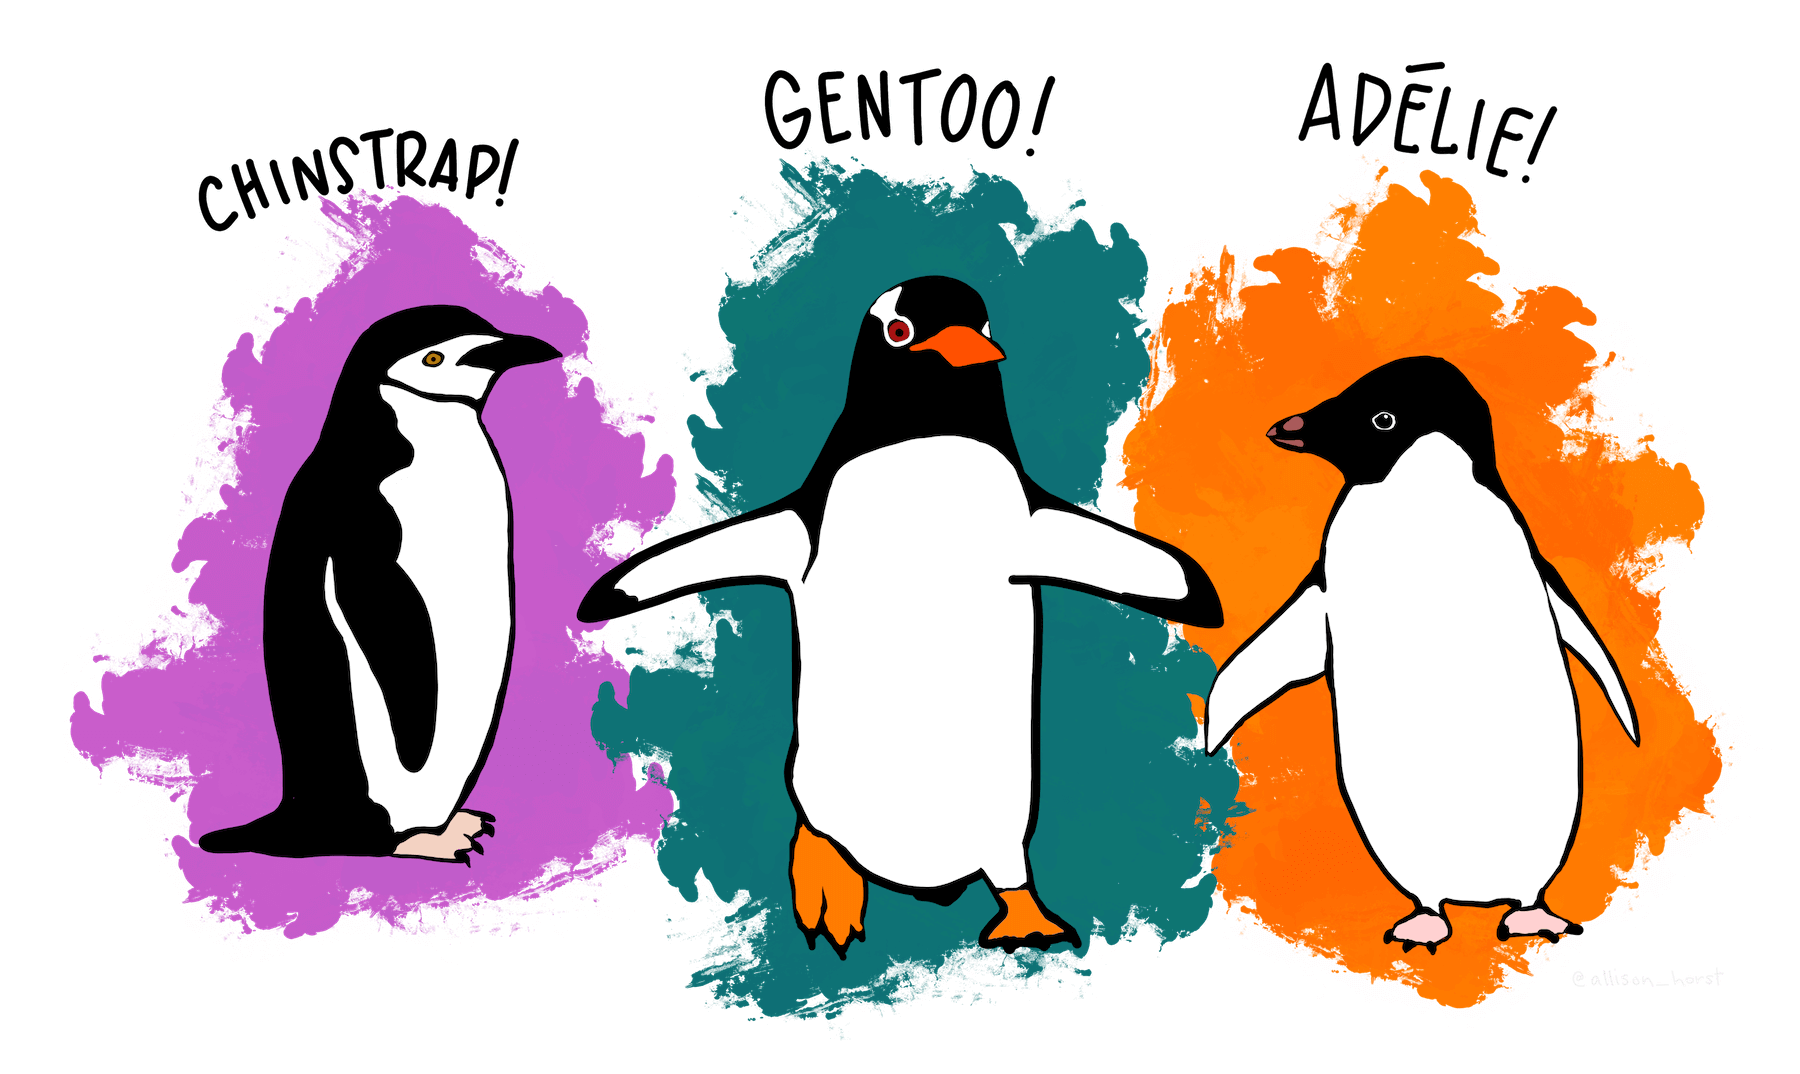
\includegraphics{fig/penguin_species.png}

}

\caption{\label{fig-penguins}Allison Horst 박사가 그린 펭귄 3종 도식화}

}

\end{minipage}%
%
\begin{minipage}[t]{0.50\linewidth}

{\centering 

\raisebox{-\height}{

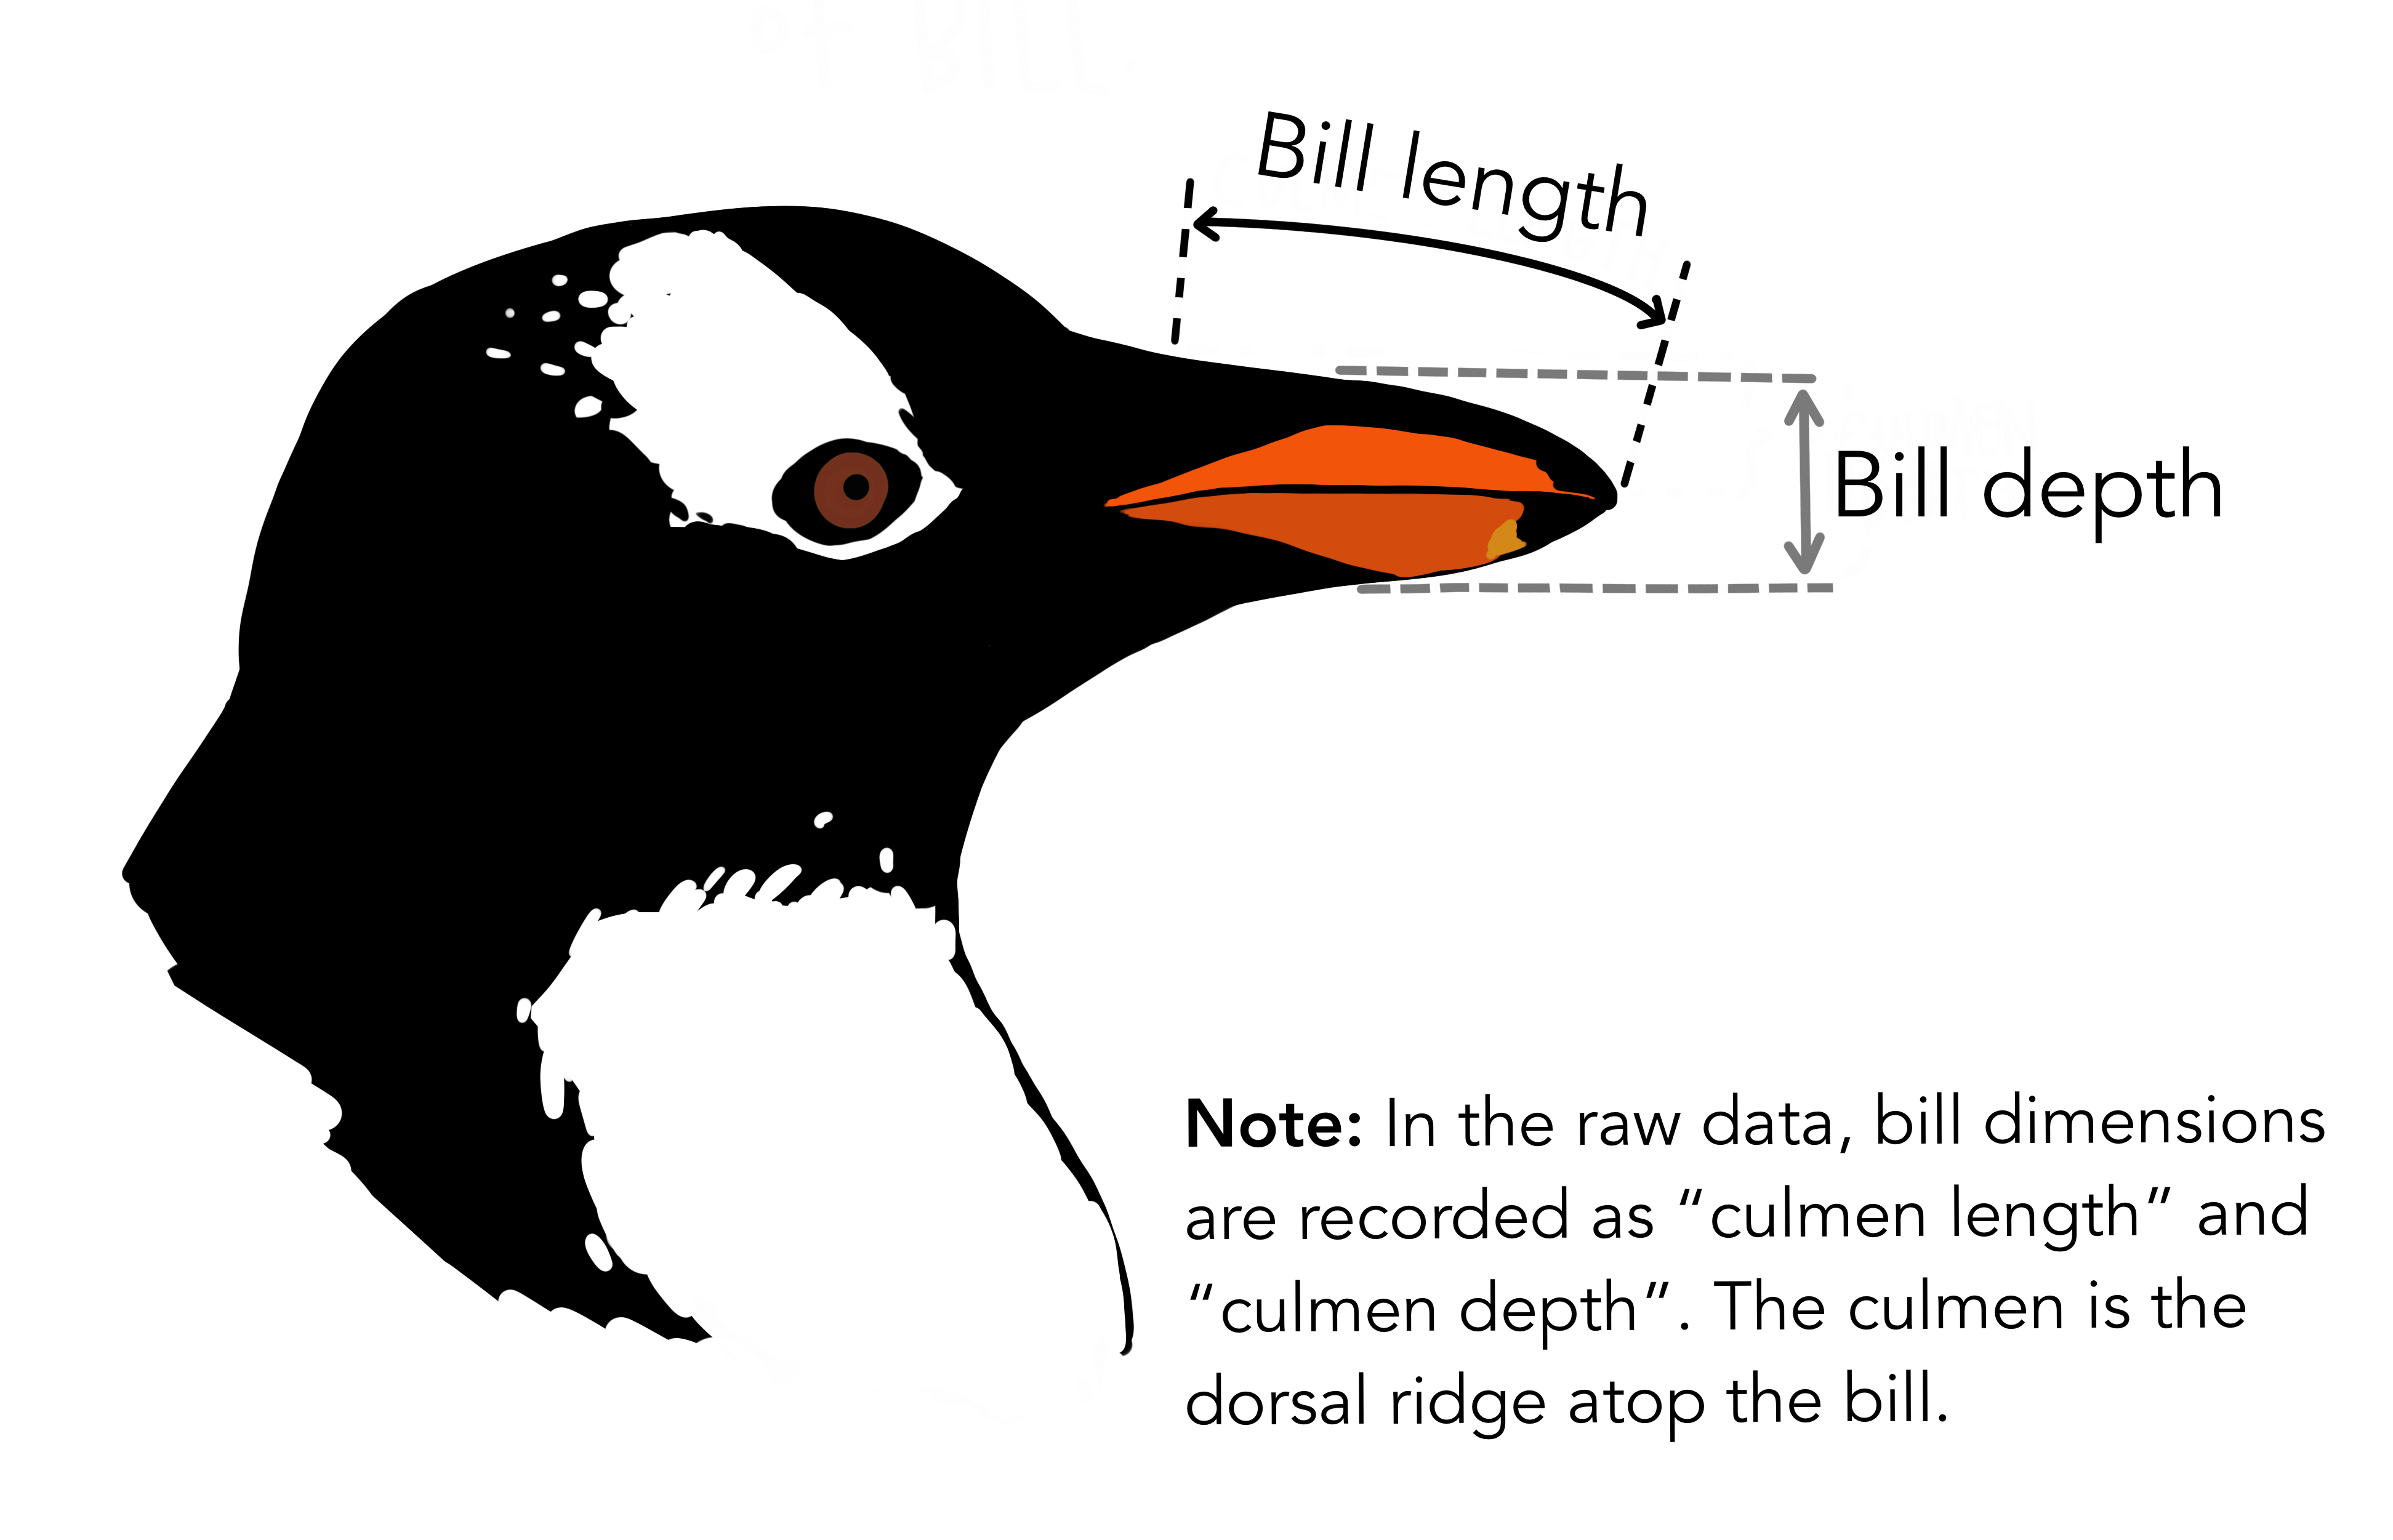
\includegraphics{fig/culmen_depth.png}

}

\caption{\label{fig-bill}펭귄 부리(bill) 변수 설명}

}

\end{minipage}%

\end{figure}

\hypertarget{r-uxcf54uxb4dc}{%
\chapter{R 코드}\label{r-uxcf54uxb4dc}}

\begin{Shaded}
\begin{Highlighting}[]
\NormalTok{mass\_flipper }\OtherTok{\textless{}{-}} \FunctionTok{ggplot}\NormalTok{(}\AttributeTok{data =}\NormalTok{ penguins,}
                       \FunctionTok{aes}\NormalTok{(}\AttributeTok{x =}\NormalTok{ flipper\_length\_mm,}
                           \AttributeTok{y =}\NormalTok{ body\_mass\_g)) }\SpecialCharTok{+}
  \FunctionTok{geom\_point}\NormalTok{(}\AttributeTok{size =} \DecValTok{3}\NormalTok{,}
             \AttributeTok{alpha =} \FloatTok{0.8}\NormalTok{) }\SpecialCharTok{+}
  \FunctionTok{theme\_minimal}\NormalTok{() }\SpecialCharTok{+}
  \FunctionTok{labs}\NormalTok{(}\AttributeTok{title =} \StringTok{"팔머 관측소 LTER 서식 펭귄 크기"}\NormalTok{,}
       \AttributeTok{subtitle =} \StringTok{"Adelie, Chinstrap, Gentoo 펭귄에 대한 물갈퀴 길이와 체질량"}\NormalTok{,}
       \AttributeTok{x =} \StringTok{"물갈퀴 길이(Flipper length) (mm)"}\NormalTok{,}
       \AttributeTok{y =} \StringTok{"체질량(Body mass) (g)"}\NormalTok{) }\SpecialCharTok{+}
  \FunctionTok{theme\_minimal}\NormalTok{()}

\NormalTok{mass\_flipper}
\end{Highlighting}
\end{Shaded}

\hypertarget{uxd45c}{%
\chapter{표}\label{uxd45c}}

\hypertarget{uxd45c-1}{%
\section{\texorpdfstring{\LaTeX 표}{표}}\label{uxd45c-1}}

\begin{tabular}{|l|l|}\hline
연령 & 빈도수 \\ \hline
18--25  & 15 \\
26--35  & 33 \\
36--45  & 22 \\ \hline
\end{tabular}

\hypertarget{gt-uxd45c}{%
\section{\texorpdfstring{\texttt{gt} 표}{gt 표}}\label{gt-uxd45c}}

\begin{Shaded}
\begin{Highlighting}[]
\NormalTok{knitr}\SpecialCharTok{::}\FunctionTok{kable}\NormalTok{(}
\NormalTok{  mtcars[}\DecValTok{1}\SpecialCharTok{:}\DecValTok{6}\NormalTok{, }\DecValTok{1}\SpecialCharTok{:}\DecValTok{10}\NormalTok{]}
\NormalTok{)}
\end{Highlighting}
\end{Shaded}

\begin{table*}

\begin{longtable}[]{@{}
  >{\raggedright\arraybackslash}p{(\columnwidth - 20\tabcolsep) * \real{0.2812}}
  >{\raggedleft\arraybackslash}p{(\columnwidth - 20\tabcolsep) * \real{0.0781}}
  >{\raggedleft\arraybackslash}p{(\columnwidth - 20\tabcolsep) * \real{0.0625}}
  >{\raggedleft\arraybackslash}p{(\columnwidth - 20\tabcolsep) * \real{0.0781}}
  >{\raggedleft\arraybackslash}p{(\columnwidth - 20\tabcolsep) * \real{0.0625}}
  >{\raggedleft\arraybackslash}p{(\columnwidth - 20\tabcolsep) * \real{0.0781}}
  >{\raggedleft\arraybackslash}p{(\columnwidth - 20\tabcolsep) * \real{0.0938}}
  >{\raggedleft\arraybackslash}p{(\columnwidth - 20\tabcolsep) * \real{0.0938}}
  >{\raggedleft\arraybackslash}p{(\columnwidth - 20\tabcolsep) * \real{0.0469}}
  >{\raggedleft\arraybackslash}p{(\columnwidth - 20\tabcolsep) * \real{0.0469}}
  >{\raggedleft\arraybackslash}p{(\columnwidth - 20\tabcolsep) * \real{0.0781}}@{}}
\toprule()
\begin{minipage}[b]{\linewidth}\raggedright
\end{minipage} & \begin{minipage}[b]{\linewidth}\raggedleft
mpg
\end{minipage} & \begin{minipage}[b]{\linewidth}\raggedleft
cyl
\end{minipage} & \begin{minipage}[b]{\linewidth}\raggedleft
disp
\end{minipage} & \begin{minipage}[b]{\linewidth}\raggedleft
hp
\end{minipage} & \begin{minipage}[b]{\linewidth}\raggedleft
drat
\end{minipage} & \begin{minipage}[b]{\linewidth}\raggedleft
wt
\end{minipage} & \begin{minipage}[b]{\linewidth}\raggedleft
qsec
\end{minipage} & \begin{minipage}[b]{\linewidth}\raggedleft
vs
\end{minipage} & \begin{minipage}[b]{\linewidth}\raggedleft
am
\end{minipage} & \begin{minipage}[b]{\linewidth}\raggedleft
gear
\end{minipage} \\
\midrule()
\endhead
Mazda RX4 & 21.0 & 6 & 160 & 110 & 3.90 & 2.620 & 16.46 & 0 & 1 & 4 \\
Mazda RX4 Wag & 21.0 & 6 & 160 & 110 & 3.90 & 2.875 & 17.02 & 0 & 1 &
4 \\
Datsun 710 & 22.8 & 4 & 108 & 93 & 3.85 & 2.320 & 18.61 & 1 & 1 & 4 \\
Hornet 4 Drive & 21.4 & 6 & 258 & 110 & 3.08 & 3.215 & 19.44 & 1 & 0 &
3 \\
Hornet Sportabout & 18.7 & 8 & 360 & 175 & 3.15 & 3.440 & 17.02 & 0 & 0
& 3 \\
Valiant & 18.1 & 6 & 225 & 105 & 2.76 & 3.460 & 20.22 & 1 & 0 & 3 \\
\bottomrule()
\end{longtable}

\end{table*}

\hypertarget{uxb370uxc774uxd130}{%
\chapter{데이터}\label{uxb370uxc774uxd130}}

\begin{tcolorbox}[enhanced jigsaw, opacityback=0, coltitle=black, left=2mm, colframe=quarto-callout-caution-color-frame, breakable, rightrule=.15mm, colbacktitle=quarto-callout-caution-color!10!white, colback=white, bottomtitle=1mm, toptitle=1mm, leftrule=.75mm, toprule=.15mm, titlerule=0mm, opacitybacktitle=0.6, title=\textcolor{quarto-callout-caution-color}{\faFire}\hspace{0.5em}{데이터 수집에 대해 궁금하신 분은 클릭하여 추가 학습하세요}, arc=.35mm, bottomrule=.15mm]
팔머펭귄 데이터는 Kristen Gorman 박사와 남국 팔머 관측소(Palmer Station,
Antarctica LTER)에서 수집되어 공공에 이용가능하게 공개되었습니다.
\end{tcolorbox}

\{palmerpenguins\} 패키지 (\protect\hyperlink{ref-palmer-penguins}{Horst
et al., 2020})를 통해 R에서 손쉽게 이용가능하게 되었고 원데이터는 Gorman
et al. (\protect\hyperlink{ref-Gorman-2014}{2014}) 에서 최초 공개되었다.


\includepdf[fitpaper]{book/canva-backmatter}

\hypertarget{refs}{}
\begin{CSLReferences}{1}{0}
\leavevmode\vadjust pre{\hypertarget{ref-Gorman-2014}{}}%
Gorman, K. B., Williams, T. D., \& Fraser, W. R. (2014). Ecological
sexual dimorphism and environmental variability within a community of
antarctic penguins (genus pygoscelis). \emph{PloS One}, \emph{9}(3),
e90081. \url{https://doi.org/10.1371/journal.pone.0090081}

\leavevmode\vadjust pre{\hypertarget{ref-palmer-penguins}{}}%
Horst, A. M., Hill, A. P., \& Gorman, K. B. (2020).
\emph{Palmerpenguins: Palmer archipelago (antarctica) penguin data}.
\url{https://allisonhorst.github.io/palmerpenguins/}

\end{CSLReferences}



\end{document}
